\documentclass[conference]{IEEEtran}
\IEEEoverridecommandlockouts
% The preceding line is only needed to identify funding in the first footnote. If that is unneeded, please comment it out.
\usepackage{cite}
\usepackage{amsmath,amssymb,amsfonts}
\usepackage{algorithm}
\usepackage[noend]{algpseudocode}
\usepackage{graphicx}
\usepackage{textcomp}
\usepackage{algorithm}
\usepackage{arevmath}     % For math symbols
\usepackage[noend]{algpseudocode}
\usepackage{tikz}
\usetikzlibrary{positioning,arrows.meta}
\usepackage{booktabs}
\usepackage{tabularx}
\usepackage{longtable}
\usepackage{array}
\usepackage{ragged2e}
\usepackage{pgfplots}
\pgfplotsset{compat=1.18}

\newcolumntype{Y}{>{\RaggedRight\arraybackslash}X}
\algrenewcommand\alglinenumber[1]{\footnotesize #1:}

% In preamble
\usepackage{tikz}
\usetikzlibrary{positioning,arrows.meta}

\newcolumntype{Y}{>{\RaggedRight\arraybackslash}X}

\title{Algorithm template}
\usepackage{xcolor}
\def\BibTeX{{\rm B\kern-.05em{\sc i\kern-.025em b}\kern-.08em
    T\kern-.1667em\lower.7ex\hbox{E}\kern-.125emX}}
\begin{document}

\title{SHARP-LLM: A Secure and Lightweight Framework for Source Code Vulnerability Analysis and Healthcare-Specific Risk Prioritization} \\
%{\footnotesize \textsuperscript{*}Note: Sub-titles are not captured in Xplore and
%should not be used}
%\thanks{Identify applicable funding agency here. If none, delete this.}
%}

\author{
\IEEEauthorblockN{Basanth M S, G Gopakumar}
\IEEEauthorblockA{
\textit{Department of Computer Science and Engineering} \\
\textit{School of Computing} \\
\textit{Amrita Vishwa Vidyapeetham} \\
Amritapuri, India
}
}

\maketitle

\begin{abstract}
Abstract— Healthcare software vulnerabilities can lead to security breaches, service disruption, patient data exposure, and regulatory risk. Early and accurate detection of vulnerable source code is therefore essential for secure and trustworthy healthcare software development. Although large language models (LLMs) have shown strong potential for source code analysis, many existing approaches rely on computationally expensive models, which limits their practical deployment. This paper presents SHARP-LLM, a secure and lightweight framework for source code vulnerability detection and risk prioritization in healthcare software using fine-tuned large language models. The framework is evaluated on the Juliet C/C++ Test Suite to identify vulnerability-relevant patterns in C/C++ programs. Beyond vulnerability detection, SHARP-LLM incorporates a healthcare-oriented risk prioritization layer that associates detected Common Weakness Enumerations (CWEs) with privacy and security risk categories and links them to policy-relevant control domains to support structured prioritization for software handling sensitive healthcare data. The experimental pipeline is implemented using Python, PyTorch, and Hugging Face, and performance is evaluated using Accuracy, Precision, Recall, F1-score, Matthews Correlation Coefficient, and False Positive Rate. Experimental results show that SHARP-LLM achieves competitive vulnerability detection performance compared with heavier state-of-the-art LLM models while reducing computational overhead, thereby supporting its practical use in real-world healthcare software environments.
\end{abstract}

\begin{IEEEkeywords}
Source code vulnerability detection, risk prioritization, healthcare software, lightweight large language models, CWE, secure software development
\end{IEEEkeywords}

\section{Introduction}

\subsection{Background and Context}
Software vulnerability detection has emerged as an important research problem at the intersection of software engineering, cybersecurity, and artificial intelligence. Its primary objective is to identify insecure coding patterns early in the software lifecycle so that defects can be corrected before deployment. This problem is especially important in healthcare, where software systems support electronic health records, telemedicine platforms, diagnostic workflows, clinical decision support, and connected medical devices. In these environments, software vulnerabilities may lead not only to system compromise and service disruption, but also to patient data exposure and regulatory risk. As a result, healthcare software development requires strong attention to both security and trustworthiness.

Despite significant progress in machine learning for source code analysis, vulnerability detection remains challenging. Vulnerabilities often arise from subtle interactions among syntax, semantics, control flow, data flow, and API usage. Consequently, two code fragments may appear structurally similar while differing substantially in security behavior. The task is further complicated by heterogeneous weakness categories, class imbalance, and the complexity of real-world codebases. Recent research has examined how machine learning and deep learning can be applied to cybersecurity tasks, including intrusion detection, malware classification, and threat analysis~\cite{vinayakumar2019ml}~\cite{vinayakumar2019ids}~\cite{babu2018review}. The findings suggest that deep learning models can capture complex patterns effectively and enhance detection performance across diverse security applications.Large language models (LLMs) have demonstrated strong potential for learning semantic properties of source code; however, many existing approaches rely on computationally expensive models that are difficult to deploy in practical secure software development workflows.

\subsection{Problem Statement}
This work addresses the problem of source code vulnerability detection in C/C++ programs using fine-tuned lightweight large language models. Given a code sample, the system is required to determine whether the sample contains vulnerability-relevant patterns and to classify it as vulnerable or non-vulnerable. In addition to detection, the work considers how identified weaknesses can be prioritized in healthcare-related software settings, where technical defects may have broader consequences for patient data protection, service continuity, and overall system trust.

Several challenges arise in this setting. First, vulnerable and non-vulnerable code may differ only in minor semantic details, such as input validation, memory handling, or access control logic. Second, vulnerability datasets typically contain diverse weakness categories with uneven distributions, which can affect model generalization. Third, high-performing models may still be impractical for continuous code analysis if they require substantial memory, inference time, or specialized hardware. These challenges motivate the development of an approach that balances detection effectiveness with computational efficiency while providing more actionable outputs for healthcare software contexts.

\subsection{Motivation}
Recent studies have shown that LLMs can improve source code analysis by capturing semantic and contextual properties more effectively than many traditional feature-engineering and deep learning approaches. However, many state-of-the-art models remain computationally intensive, which limits their suitability for routine deployment in environments that require repeated scanning, timely feedback, and practical resource usage. This creates a clear need for secure and lightweight approaches that preserve useful detection capability while reducing computational overhead.

A second motivation arises from the limitations of purely technical vulnerability classification. In healthcare software, vulnerability findings are not equally important; some may pose higher risks because they affect sensitive data handling, service availability, or safety-critical workflows. Therefore, beyond identifying whether code is vulnerable, there is value in prioritizing findings according to healthcare-oriented risk factors. Such prioritization can support more effective remediation and help developers focus first on the most consequential weaknesses.

\subsection{Objectives}
The primary objective of this work is to design and evaluate \textit{SHARP-LLM}(\textbf{S}ecure \textbf{H}ealthcare Code Vulnerability \textbf{A}nalysis and \textbf{R}isk \textbf{P}rioritization using Lightweight \textbf{L}arge \textbf{L}anguage \textbf{M}odels), a secure and lightweight framework for source code vulnerability detection and risk prioritization in healthcare software. More specifically, the study aims to analyze C/C++ source code using a fine-tuned lightweight LLM, identify vulnerability-relevant patterns, and evaluate model performance using standard classification metrics, including Accuracy, Precision, Recall, F1-score, Matthews Correlation Coefficient, and False Positive Rate. Another objective is to compare the proposed framework with heavier state-of-the-art LLM models in order to assess whether competitive detection performance can be achieved with lower computational overhead. A further objective is to extend vulnerability detection with a healthcare-oriented risk prioritization layer that supports structured ranking of detected weaknesses for software handling sensitive healthcare data.

\subsection{Contributions}
The contributions of this work are as follows. First, it presents \textit{SHARP-LLM}, a secure and lightweight framework for source code vulnerability detection in healthcare software using fine-tuned large language models. Second, it evaluates the framework on the Juliet C/C++ Test Suite, a standard benchmark for software weakness detection, to identify vulnerability-relevant patterns in C/C++ programs. Third, it introduces a healthcare-oriented risk prioritization layer that associates detected Common Weakness Enumerations (CWEs) with privacy and security risk categories and links them to policy-relevant control domains to support structured prioritization of vulnerability findings. Finally, it demonstrates that the proposed framework achieves competitive vulnerability detection performance relative to heavier state-of-the-art LLM models while reducing computational overhead, thereby improving practical deployability.

\subsection{System / Functionality Diagram}
Figure~\ref{fig:system_pipeline} illustrates the overall workflow of SHARP-LLM. The pipeline begins with C/C++ source code input, followed by preprocessing and tokenization. The processed code is then analyzed by a fine-tuned lightweight LLM, which produces vulnerability predictions. When a vulnerability is identified, the result is associated with the relevant CWE category and passed to a healthcare-oriented risk prioritization layer. This layer interprets the detected weakness in terms of privacy and security risk categories and links the finding to policy-relevant control domains to support structured prioritization. The final output provides ranked vulnerability findings for healthcare software environments.

\begin{figure}[t]
\centering
\resizebox{\columnwidth}{!}{%
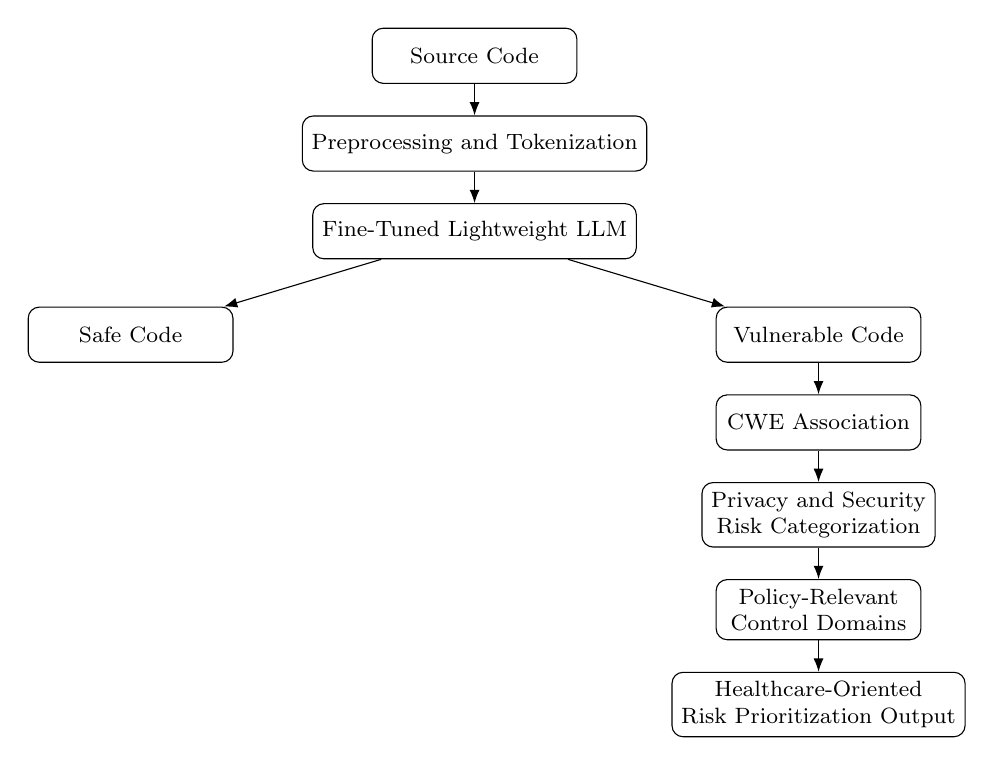
\begin{tikzpicture}[
    node distance=4mm and 6mm,
    block/.style={
        draw,
        rounded corners,
        align=center,
        minimum width=2.6cm,
        minimum height=0.7cm,
        font=\footnotesize
    },
    line/.style={-Latex, thin}
]

\node[block] (input) {Source Code};
\node[block, below=of input] (prep) {Preprocessing and Tokenization};
\node[block, below=of prep] (llm) {Fine-Tuned Lightweight LLM};

\node[block, below left=6mm and 10mm of llm] (safe) {Safe Code};
\node[block, below right=6mm and 10mm of llm] (vuln) {Vulnerable Code};

\node[block, below=of vuln] (cwe) {CWE Association};
\node[block, below=of cwe] (risk) {Privacy and Security\\Risk Categorization};
\node[block, below=of risk] (policy) {Policy-Relevant\\Control Domains};
\node[block, below=of policy] (output) {Healthcare-Oriented\\Risk Prioritization Output};

\draw[line] (input) -- (prep);
\draw[line] (prep) -- (llm);
\draw[line] (llm) -- (safe);
\draw[line] (llm) -- (vuln);
\draw[line] (vuln) -- (cwe);
\draw[line] (cwe) -- (risk);
\draw[line] (risk) -- (policy);
\draw[line] (policy) -- (output);

\end{tikzpicture}%
}
\caption{High-level workflow of the proposed SHARP-LLM framework.}
\label{fig:system_pipeline}
\end{figure}

\section{Literature Review}

Software vulnerability detection has evolved from traditional static analysis and rule-based methods to machine learning, deep learning, and, more recently, large language model (LLM)-based approaches. Survey studies by Dolcetti and Iotti~\cite{dolcetti2025}, Shaon and Akter~\cite{shaon2025}, and Taghavi Far and Feyzi~\cite{taghavifar2025} show that LLMs have significantly expanded the capability of automated code analysis by capturing semantic and contextual properties that are difficult to model using handcrafted rules alone. At the same time, these reviews consistently report persistent challenges, including false positives, limited generalization across projects, lack of interpretability, dataset imbalance, and the high computational cost of modern LLM-based methods. These findings establish the broader need for practical and reliable vulnerability detection frameworks.

A large body of recent work has focused on improving vulnerability detection accuracy by enriching code representations or combining LLMs with complementary reasoning mechanisms. Lu et al.~\cite{lu2024} proposed GRACE, which integrates graph structural information with LLM analysis to better capture code dependencies and reported strong F1-score improvements on benchmark datasets. Zhang et al.~\cite{zhang2025} introduced VulTrLM, which decomposes abstract syntax trees into smaller units enriched with LLM-generated comments, thereby improving semantic understanding of complex code. Tian et al.~\cite{tian2025} proposed FUSEVUL, a multi-modal approach that combines source code semantics with natural language explanations, demonstrating that textual reasoning cues can improve vulnerability detection performance, particularly in low-resource settings. These studies confirm that incorporating structure, semantics, and auxiliary reasoning can strengthen vulnerability detection beyond simple token-based modeling.

Another important line of work addresses explainability and developer-facing usefulness. Mao et al.~\cite{mao2025} proposed LLMVulExp, a teacher-student framework for explainable vulnerability detection, while Chen et al.~\cite{chen2026} introduced GPTVD, which combines static slicing with chain-of-thought prompting for finer-grained and more interpretable analysis. Yang et al.~\cite{yang2025} further showed through DLAP that combining deep learning signals with LLM prompting can improve both cost-effectiveness and explanation quality. These studies are relevant because they move vulnerability detection beyond binary prediction and highlight the importance of outputs that can support downstream developer action.

In parallel, several studies have examined how to improve deployment efficiency and reduce the cost of LLM-based vulnerability analysis. Liu et al.~\cite{liu2025} explored model compression through knowledge distillation and LoRA in VulACLLM, showing that lightweight strategies can substantially reduce training time and memory usage while retaining useful detection capability. Ferrag et al.~\cite{ferrag2025} introduced SecureFalcon, a compact vulnerability classification model that achieved strong binary and multiclass performance with faster inference. These studies are particularly relevant to the proposed work because they demonstrate that lightweight models can provide competitive vulnerability detection performance without requiring the full computational burden of very large LLMs.

Recent research has also explored contextual and adaptive vulnerability detection. Qiu et al.~\cite{qiu2026} proposed RLV, which enhances function-level vulnerability detection by incorporating project-level context such as callers, callees, and data types. Zheng et al.~\cite{zheng2024} addressed data scarcity through Few-VulD, a few-shot learning framework that adapts to new tasks with limited labeled data. Hinrichs et al.~\cite{hinrichs2025} showed that prompt phrasing itself can significantly influence LLM vulnerability predictions, emphasizing the sensitivity of conversational models to prompt design. Ciavatta et al.~\cite{ciavatta2026} compared LLMs with traditional static analysis tools and observed that their usefulness depends strongly on the deployment context and tolerance for false positives. Together, these studies indicate that performance alone is not sufficient; robustness, context awareness, and deployment practicality also matter.

Although the above studies advance vulnerability detection substantially, most of them remain focused on general-purpose software security rather than domain-specific prioritization. This limitation is particularly important for healthcare software, where not all vulnerabilities have the same operational significance. Weaknesses affecting patient data handling, safety-relevant workflows, or service continuity may require higher remediation priority than general coding defects. In this context, Ameh et al.~\cite{ameh2025} developed C3-VULMAP, a privacy-aware vulnerability dataset for healthcare systems that maps vulnerabilities to LINDDUN privacy threat types and CWE categories. This work is especially relevant because it highlights the need for healthcare-oriented and privacy-aware vulnerability analysis rather than generic classification alone.

Despite these advances, three important gaps remain. First, many existing LLM-based methods continue to rely on computationally expensive architectures, which limits routine deployment in secure software development workflows. Second, much of the current literature focuses on vulnerability detection accuracy without adequately addressing how detected findings should be prioritized in domain-specific settings such as healthcare. Third, healthcare-oriented and privacy-aware vulnerability resources remain comparatively limited when compared with the broader general-purpose vulnerability detection literature. These gaps motivate the proposed \textit{SHARP-LLM} framework, which combines secure and lightweight source code vulnerability detection with a healthcare-oriented risk prioritization layer. In this way, the proposed work aims to bridge the gap between efficient LLM-based vulnerability detection and structured prioritization of findings for software handling sensitive healthcare data.

% -------- Corrected Conference-friendly Comparison Table --------
\begin{table*}[!t]
\centering
\scriptsize
\setlength{\tabcolsep}{2.5pt}
\renewcommand{\arraystretch}{1.12}

\begin{tabular}{@{}c
>{\RaggedRight\arraybackslash}p{1.55cm}
>{\RaggedRight\arraybackslash}p{2.00cm}
>{\RaggedRight\arraybackslash}p{2.15cm}
>{\RaggedRight\arraybackslash}p{2.45cm}
c
c
>{\RaggedRight\arraybackslash}p{2.55cm}@{}}
\toprule
\textbf{Paper} &
\textbf{Framework} &
\textbf{Core Focus} &
\textbf{Input / Representation} &
\textbf{LLM / Model Strategy} &
\textbf{Eff.} &
\textbf{Health / Risk} &
\textbf{Key Limitation} \\
\midrule

Lu et al. (2024)~\cite{lu2024} &
GRACE &
Graph-enhanced vulnerability detection &
Source code + graph structure &
Graph-augmented prompting with similarity-based ICL &
No &
No &
Prompt sensitivity and limited language coverage \\

Yang et al. (2025)~\cite{yang2025} &
DLAP &
DL-guided prompting for detection and explanation &
Source code + DL outputs &
DL predictions used to construct LLM prompts &
Partial &
No &
Strong dependence on DL model quality \\

Tian et al. (2025)~\cite{tian2025} &
FUSEVUL &
Multi-modal vulnerability detection &
Code semantics + natural language explanations &
Explanation-aware fusion with pretrained encoders and self-attention &
No &
No &
Limited mainly to C/C++ and basic prompting \\

Mao et al. (2025)~\cite{mao2025} &
LLMVulExp &
Explainable vulnerability detection &
Raw code + key-code extraction &
Teacher-student framework with CoT prompting and LoRA fine-tuning &
Partial &
No &
High annotation and computational cost \\

Liu et al. (2025)~\cite{liu2025} &
VulACLLM &
Efficient vulnerability detection &
AST + CFG + source code &
Hybrid structural features with LoRA / knowledge distillation &
Yes &
No &
Performance trade-off due to compression \\

Ferrag et al. (2025)~\cite{ferrag2025} &
SecureFalcon &
Lightweight vulnerability classification &
Source code &
Compact fine-tuned LLM for binary and multiclass detection &
Yes &
No &
Limited to known patterns and C/C++ training data \\

Qiu et al. (2026)~\cite{qiu2026} &
RLV &
Context-aware vulnerability detection &
Source code + repository context &
Retrieval and refinement prompting without task-specific fine-tuning &
Partial &
No &
Context-length limits and function-level restriction \\

Chen et al. (2026)~\cite{chen2026} &
GPTVD &
Fine-grained, interpretable detection &
Threat code slices + code context &
Static slicing with ICL and chain-of-thought prompting &
No &
No &
Limited dataset support and scalability concerns \\

Ameh et al. (2025)~\cite{ameh2025} &
C3-VULMAP &
Privacy-aware healthcare vulnerability dataset &
Healthcare-related C/C++ functions mapped to CWE and LINDDUN &
Dataset resource for privacy-aware vulnerability analysis &
N/A &
Yes &
Resource-intensive construction and current language limitation \\

This work &
SHARP-LLM &
Secure and lightweight detection with healthcare-oriented prioritization &
Source code + CWE findings + healthcare risk attributes &
Fine-tuned lightweight LLM with structured risk-prioritization layer &
Yes &
Yes &
Dependent on benchmark coverage and risk-mapping quality \\

\bottomrule
\end{tabular}

\caption{Comparison of selected frameworks and resources relevant to SHARP-LLM.}
\label{tab:comparison_sharp}
\end{table*}

% ===========================================================================
% Section 5 — Solution Approach / Methodology
% ===========================================================================

\section{Solution Approach / Methodology}
\label{sec:methodology}

This paper proposes the \textbf{SHARP-LLM} framework for automated source code
vulnerability detection and CWE classification.  The framework leverages
fine-tuned lightweight large language models operating on tokenised C/C++
source code to classify vulnerabilities into 118~CWE categories.  The
novelty of the approach is threefold: (i)~a \emph{template-aware data
splitting} strategy that eliminates structural data leakage inherent in the
Juliet Test Suite; (ii)~a \emph{multi-paradigm model evaluation} that
systematically compares encoder-based fine-tuning, QLoRA-based
parameter-efficient fine-tuning, and zero-shot generative inference within a
single unified pipeline; and (iii)~a healthcare-oriented risk
prioritisation layer that maps detected CWE categories to privacy, security,
and policy-relevant control domains.

% ---------------------------------------------------------------------------
\subsection{Pipeline Overview}
\label{sec:pipeline}

Fig.~\ref{fig:system_pipeline} presents the end-to-end SHARP-LLM pipeline.
Raw C/C++ source code first undergoes preprocessing and sub-word
tokenisation.  The tokenised representation is then fed into one of several
fine-tuned lightweight LLMs.  The model produces a binary safe/vulnerable
decision; for vulnerable inputs the system further performs multi-class CWE
association across 118~categories, maps the identified CWE to privacy and
security risk categories, aligns the risk with policy-relevant control
domains, and finally outputs a healthcare-oriented risk prioritisation
score.

% ---------------------------------------------------------------------------
\subsection{Data and Environment Design}
\label{sec:data_design}

\subsubsection{Dataset}
The study employs the \textbf{NIST Juliet Test Suite for C/C++ v1.3}~\cite{juliet2017}, a widely used benchmark containing synthetic but
structurally realistic test cases spanning 118~Common Weakness Enumeration
(CWE) categories.  Each source file follows a naming convention encoding the
CWE identifier, functional variant, and flow variant, which we parse using a
regular-expression extractor utility.  The resulting dataset comprises individual \texttt{.c}/\texttt{.cpp}
files, each labelled by CWE category and template identifier.

\subsubsection{Input Representation and Feature Space}
Each sample is a raw C/C++ source code string.  Preprocessing applies a
four-stage pipeline:
\begin{enumerate}
    \item \textbf{Header removal} --- strips the auto-generated
          \texttt{TEMPLATE GENERATED TESTCASE FILE} comment block.
    \item \textbf{Comment stripping} --- a character-level state machine
          removes single-line (\texttt{//}) and multi-line
          (\texttt{/* ... */}) comments while preserving string and
          character literals.
    \item \textbf{Guard removal} --- eliminates Juliet-specific preprocessor
          guards (\texttt{\#ifndef OMITBAD}, \texttt{\#ifndef OMITGOOD},
          \texttt{\#ifdef INCLUDEMAIN}, and trailing \texttt{\#endif}).
    \item \textbf{Whitespace normalisation} --- collapses consecutive
          whitespace and blank lines to produce a compact, semantics-preserving
          representation.
\end{enumerate}
The preprocessed code is tokenised on-the-fly using each model's native
sub-word tokeniser (SentencePiece for CodeT5 family, byte-pair encoding for
CodeBERT/GraphCodeBERT, Gemma tokeniser for CodeGemma), with a maximum
sequence length of $L = 256$ tokens, right-truncation, and
\texttt{max\_length} padding.

\subsubsection{Output Space}
The output is a 118-dimensional probability vector $\hat{\mathbf{y}} \in
\mathbb{R}^{118}$ produced via a softmax layer.  Each dimension corresponds
to one CWE category, mapped through a deterministic label encoding (CWE IDs
sorted numerically $\mapsto$ integer labels $0 \ldots 117$).  At inference
time the top-$k$ predictions with associated confidence scores are returned.

\subsubsection{Template-Aware Data Splitting}
A key design decision is the \emph{template-aware splitting} strategy.  In
the Juliet suite, each CWE category contains multiple \emph{templates}
(functional variants) instantiated across several \emph{flow variants}.
Flow variants of the same template share identical vulnerability logic,
differing only in control-flow structure.  A na\"ive random split risks
placing flow variants of the same template in both train and test sets,
causing structural data leakage and artificially inflated metrics.

We employ \texttt{GroupShuffleSplit} from scikit-learn with the template
identifier as the grouping key, performed independently within each CWE
category to maintain class balance:
\begin{equation}
    \forall\, t \in \mathcal{T}: \quad t \in \mathcal{D}_{\text{train}}
    \;\oplus\; t \in \mathcal{D}_{\text{test}}
\label{eq:template_split}
\end{equation}
where $\mathcal{T}$ is the set of all template identifiers and $\oplus$
denotes exclusive disjunction.  CWE categories with only a single template
are assigned entirely to the training set.  The split ratio is 80/20
(train/test) with a fixed random seed for reproducibility.

% ---------------------------------------------------------------------------
\subsection{Model Architectures}
\label{sec:model}

The framework evaluates three distinct model paradigms, enabling a
systematic comparison of fine-tuning strategies under resource-constrained
environments.

\subsubsection{Encoder-Based Classification}
Four pre-trained encoder models are fine-tuned with a classification head:

\begin{itemize}
    \item \textbf{CodeT5-Small} (60\,M params) and \textbf{CodeT5-Base}
          (220\,M params)~\cite{wang2021codet5}: T5-family encoder-decoder
          models pre-trained on CodeSearchNet with bimodal dual generation
          and identifier-aware objectives.  We use only the encoder.
    \item \textbf{CodeBERT-Base} (125\,M params)~\cite{feng2020codebert}:
          RoBERTa-based model pre-trained on programming and natural
          language with masked language modelling and replaced token
          detection.
    \item \textbf{GraphCodeBERT-Base} (125\,M params)~\cite{guo2020graphcodebert}:
          extends CodeBERT with data-flow graph pre-training objectives.
\end{itemize}

The classification architecture is:
\begin{equation}
    \hat{\mathbf{y}} = \text{softmax}\!\Big(
        \mathbf{W} \cdot \text{Dropout}\!\big(
            \bar{\mathbf{h}}
        \big) + \mathbf{b}
    \Big)
\label{eq:classifier}
\end{equation}
where $\bar{\mathbf{h}}$ is the mean-pooled encoder output over non-padding
tokens:
\begin{equation}
    \bar{\mathbf{h}} = \frac{
        \sum_{i=1}^{L} m_i \cdot \mathbf{h}_i
    }{
        \sum_{i=1}^{L} m_i
    }
\label{eq:mean_pool}
\end{equation}
with $\mathbf{h}_i \in \mathbb{R}^{d}$ being the hidden state at position
$i$, $m_i \in \{0,1\}$ the attention mask, and $d$ the model's hidden
dimension.

\subsubsection{QLoRA-Based Parameter-Efficient Fine-Tuning}
For larger decoder-only models, we employ Quantised Low-Rank Adaptation
(QLoRA)~\cite{dettmers2023qlora} applied to \textbf{CodeGemma-2B}
(v1.1, 2.5\,B parameters)~\cite{team2024codegemma}, a model
purpose-built for code tasks with dependency-graph and unit-test
lexical packing during pre-training.

The base model is loaded with 4-bit NormalFloat (NF4) quantisation via
\texttt{BitsAndBytesConfig} with double quantisation enabled, reducing
memory from $\approx\!5.5$\,GB (FP16) to $\approx\!1.8$\,GB.  Low-rank
adapters are applied to all linear projection layers:
\begin{equation}
    \mathbf{W}' = \mathbf{W}_{\text{frozen}}^{\text{NF4}}
                 + \frac{\alpha}{r}\,\mathbf{B}\mathbf{A}
\label{eq:lora}
\end{equation}
where $\mathbf{W}_{\text{frozen}}^{\text{NF4}}$ is the 4-bit quantised
weight matrix, $\mathbf{B} \in \mathbb{R}^{d \times r}$ and
$\mathbf{A} \in \mathbb{R}^{r \times k}$ are the low-rank adapter
matrices with rank $r = 16$ and scaling factor $\alpha = 32$.  Target
modules include query, key, value, output, gate, up, and down projections.
The classification head (\texttt{score} layer) is trained in full
precision via \texttt{modules\_to\_save}.

Table~\ref{tab:qlora_config} summarises the QLoRA configuration.

\begin{table}[H]
\centering
\caption{QLoRA configuration for CodeGemma-2B fine-tuning.}
\label{tab:qlora_config}
\small
\setlength{\tabcolsep}{6pt}
\renewcommand{\arraystretch}{1.08}
\begin{tabular}{ll}
\toprule
\textbf{Parameter} & \textbf{Value} \\
\midrule
LoRA rank ($r$)        & 16 \\
LoRA alpha ($\alpha$)  & 32 \\
LoRA dropout           & 0.05 \\
Target modules         & q, k, v, o, gate, up, down \\
Quantization type      & NF4 (double quant.) \\
Compute dtype          & bfloat16 \\
Gradient checkpointing & Enabled \\
Optimizer              & PagedAdamW (8-bit) \\
Learning rate          & $2 \times 10^{-4}$ \\
Effective batch size   & 8 ($2 \times 4$ accum.) \\
Epochs                 & 5 (patience = 2) \\
\bottomrule
\end{tabular}
\end{table}

\subsubsection{Zero-Shot Generative Inference}
Two generative models are evaluated without any training:
\textbf{CodeGemma-2B}~\cite{team2024codegemma} (completion mode) and
\textbf{Gemma-4-E2B-IT}~\cite{team2024gemma} (instruction-tuned mode, 5.1\,B
total parameters, 2.3\,B effective).

Zero-shot inference uses a structured prompt that enumerates all 118~valid
CWE identifiers and instructs the model to output only the CWE number.
For instruction-tuned models, prompts are wrapped with the model's chat
template.  Beam search ($B = 10$ for CodeGemma, $B = 2$ for Gemma~4~IT) is
used for decoding, with a regex-based parser extracting valid CWE numbers
from each beam.  Confidence scores are derived via softmax normalisation
of beam log-probabilities:
\begin{equation}
    c_j = \frac{\exp(s_j)}{\sum_{j'=1}^{K} \exp(s_{j'})}
\label{eq:beam_confidence}
\end{equation}
where $s_j$ is the log-probability of the $j$-th valid beam and $K$ is the
number of unique valid predictions.

% ---------------------------------------------------------------------------
\subsection{Novel Components}
\label{sec:novel}

\subsubsection{Template-Aware Anti-Leakage Splitting}
Existing studies on the Juliet Test Suite often perform random sample-level
splitting, which introduces template leakage --- flow variants of the same
template appearing in both train and test sets.  Since flow variants share
identical vulnerability logic, this inflates reported metrics.  Our
template-aware splitting (Section~\ref{sec:data_design}) enforces strict
separation at the template level, providing a more rigorous evaluation.

\subsubsection{Multi-Paradigm Comparative Framework}
Rather than evaluating a single model or fine-tuning strategy, SHARP-LLM
provides a unified pipeline for comparing three paradigms ---
encoder-based full fine-tuning, QLoRA parameter-efficient fine-tuning, and
zero-shot generative inference --- under identical data conditions,
preprocessing, and evaluation metrics.  This enables controlled ablation
of model architecture and training strategy effects.

\subsubsection{Resource-Constrained QLoRA Integration}
The QLoRA fine-tuning of CodeGemma-2B is specifically engineered for
consumer-grade hardware (8\,GB VRAM), demonstrating that decoder-based
models with 2.5\,B parameters can be fine-tuned for multi-class
vulnerability classification on a single GPU.  The combination of NF4
double quantisation, gradient checkpointing, 8-bit paged optimiser, and
adapter-only training reduces peak VRAM consumption to
$\approx\!3$--$4$\,GB.

% ---------------------------------------------------------------------------
\subsection{Training Procedure}
\label{sec:training}

\subsubsection{Encoder Model Training}
All encoder models are trained with the AdamW optimiser~\cite{loshchilov2019decoupled} using a learning
rate of $5 \times 10^{-5}$, weight decay of $0.01$, and dropout
$p = 0.1$.  The loss function is the standard cross-entropy:
\begin{equation}
    \mathcal{L} = -\frac{1}{N}\sum_{i=1}^{N}\sum_{c=1}^{C}
        y_{i,c} \log \hat{y}_{i,c}
\label{eq:ce_loss}
\end{equation}
where $N$ is the batch size and $C = 118$ is the number of classes.
Mixed-precision training (FP16) with gradient scaling is enabled on CUDA
devices.  Early stopping monitors the macro-F1 score on the test set with a
patience of 1~epoch.

\subsubsection{QLoRA Training}
The QLoRA training loop follows a similar structure but operates only on
the trainable parameters (LoRA adapters and the classification head,
$\approx\!0.5\%$ of total parameters).  The 8-bit PagedAdamW optimiser
is used with a higher learning rate ($2 \times 10^{-4}$) appropriate for
adapter tuning.  Mixed-precision uses bfloat16 (preferred for NF4 QLoRA
stability).  Gradient accumulation over 4~steps yields an effective batch
size of $8$.  Early stopping patience is set to 2~epochs, and the maximum
number of epochs is $5$.

\subsubsection{Evaluation Metrics}
All models are evaluated using the following macro-averaged metrics:
\begin{itemize}
    \item \textbf{Accuracy}: $\frac{1}{N}\sum_{i=1}^{N}
          \mathbb{1}[\hat{y}_i = y_i]$
    \item \textbf{Macro Precision, Recall, F1-Score}: averaged
          across all 118 classes with zero-division fallback
    \item \textbf{Matthews Correlation Coefficient (MCC)}: a balanced
          measure robust to class imbalance
    \item \textbf{Macro False Positive Rate (FPR)}: computed per-class
          from the confusion matrix:
          $\text{FPR}_c = \frac{\text{FP}_c}{\text{FP}_c + \text{TN}_c}$,
          then averaged
    \item \textbf{Inference Latency}: average over 20 forward passes
          (5-run warmup, CUDA synchronised)
\end{itemize}

% ---------------------------------------------------------------------------
\subsection{Algorithm / Pseudocode}
\label{sec:pseudocode}

Algorithm~\ref{alg:sharp_llm} presents SHARP-LLM: Vulnerability Detection and Risk Prioritization.

\begin{algorithm}[t]
\caption{SHARP-LLM: Vulnerability Detection and Risk Prioritization}
\label{alg:sharp_llm}
\begin{algorithmic}[1]
\Require Source code sample $x$
\Ensure Vulnerability label $\hat{y}$, detected CWE $c$, risk categories $R$, control domains $D$, priority score $P$, priority level $L$

\State $x' \gets \textsc{PreprocessCode}(x)$ \Comment{normalize, tokenize, prepare source code}

\State $(\hat{y}, s) \gets \textsc{DetectVulnerability}(x')$ \Comment{$\hat{y}$: predicted label, $s$: confidence}

\If{$\hat{y} = \text{non-vulnerable}$}
    \State \Return $(\hat{y}, \emptyset, \emptyset, \emptyset, 0, \text{Low})$
\EndIf

\State $c \gets \textsc{AssociateCWE}(x', \hat{y})$

\State $R \gets \textsc{MapToRiskCategories}(c)$

\State $D \gets \textsc{LinkToControlDomains}(R)$

\State $E \gets \textsc{EstimateTechnicalSeverity}(c)$
\State $H \gets \textsc{EstimateHealthcareImpact}(R, D)$
\State $P \gets w_1 s + w_2 E + w_3 H$
\State $L \gets \textsc{AssignPriorityLevel}(P)$

\State \Return $(\hat{y}, c, R, D, P, L)$
\end{algorithmic}
\end{algorithm}

\subsection{Privacy and Security Risk Categorization}
After vulnerability detection, SHARP-LLM categorizes each detected weakness into privacy and security risk classes to support healthcare-oriented prioritization. This step is motivated by the fact that vulnerabilities in healthcare software may affect patient-data confidentiality, traceability, service continuity, and compliance obligations differently. To provide a structured interpretation of these differences, the framework adopts the healthcare-specific perspective introduced by C3-VULMAP~\cite{ameh2025}, which maps healthcare-related software weaknesses to both CWE categories and LINDDUN privacy threat types.

In SHARP-LLM, the detected Common Weakness Enumeration (CWE) serves as the starting point for this categorization. Using a C3-VULMAP-inspired mapping, the framework associates each detected CWE with one or more privacy and security threat classes, including linkability, identifiability, non-repudiation, detectability, information disclosure, unawareness, and non-compliance. This enables the framework to reinterpret a technical vulnerability finding as a healthcare-relevant risk signal rather than as a purely code-level defect.

Let $c_i$ denote the CWE assigned to code instance $x_i$. The corresponding risk category set is computed as
\begin{equation}
R_i = f(c_i),
\end{equation}
where $f(\cdot)$ denotes the healthcare-oriented risk mapping function and $R_i$ represents the resulting privacy and security risk categories. These categories are then used in the subsequent prioritization stage to derive broader impact attributes, such as patient-data exposure risk, service availability impact, and policy-relevant control relevance.

This categorization stage is used to support prioritization, not direct legal classification. Its purpose is to provide an interpretable bridge between vulnerability detection and healthcare-oriented decision support. By incorporating this step, SHARP-LLM moves beyond binary vulnerability prediction and offers a more structured basis for ranking vulnerabilities in software systems that process sensitive healthcare data.

\subsection{Policy-Relevant Control Domains}
Following privacy and security risk categorization, SHARP-LLM links each detected weakness to policy-relevant control domains in order to support healthcare-oriented prioritization. This step is motivated by the fact that vulnerabilities in healthcare software may affect not only technical security properties, but also broader control expectations related to patient-data protection, access management, auditability, service continuity, and secure handling of sensitive information. Therefore, after the detected Common Weakness Enumeration (CWE) is mapped to one or more privacy and security risk categories, the framework further interprets the finding in terms of the control areas that are most likely to be affected.

This mapping is informed by the healthcare-oriented privacy perspective provided by C3-VULMAP~\cite{ameh2025}. Since C3-VULMAP associates healthcare-related software vulnerabilities with both CWE categories and LINDDUN privacy threat types, it provides a useful basis for connecting technical weaknesses with broader privacy and security concerns. In SHARP-LLM, the risk categories obtained in the previous stage are used to identify policy-relevant control domains such as confidentiality protection, access control, audit and accountability, secure data handling, and service availability. For example, weaknesses associated with information disclosure may be linked to confidentiality and secure data handling domains, while weaknesses related to unawareness or non-compliance may be linked to transparency, accountability, or governance-oriented control areas.

Let $R_i$ denote the privacy and security risk-category set assigned to a vulnerable code instance $x_i$. A control-domain mapping function $g(\cdot)$ is then applied as
\begin{equation}
C_i = g(R_i),
\end{equation}
where $C_i$ denotes the set of policy-relevant control domains associated with the detected weakness. These control domains do not represent a direct legal judgment. Instead, they provide a structured interpretation layer that helps translate technical vulnerability findings into healthcare-relevant control implications.

The purpose of this stage is to strengthen the final prioritization process. By associating each detected vulnerability with policy-relevant control domains, SHARP-LLM provides a more actionable view of the potential impact of a weakness in healthcare software environments. This enables the framework to move beyond generic vulnerability detection and support remediation decisions that are better aligned with privacy, security, and operational priorities in systems handling sensitive healthcare data.

\subsection{Risk Prioritization}
After identifying the vulnerability class, assigning privacy and security risk categories, and linking the finding to policy-relevant control domains, SHARP-LLM performs a final risk prioritization step. The goal of this stage is to rank detected vulnerabilities according to their likely importance in healthcare software environments, where not all weaknesses have the same operational impact. In particular, vulnerabilities affecting sensitive healthcare data, service continuity, access control, or safety-relevant workflows should be prioritized more highly than weaknesses with lower practical consequence.

The proposed prioritization mechanism combines technical and healthcare-oriented factors into a single risk score. Let $x_i$ denote a code instance classified as vulnerable, and let $c_i$, $R_i$, and $C_i$ denote its associated CWE category, privacy and security risk-category set, and policy-relevant control-domain set, respectively. A prioritization function $h(\cdot)$ is then defined as
\begin{equation}
P_i = h(c_i, R_i, C_i, s_i),
\end{equation}
where $P_i$ is the final priority score and $s_i$ is the model confidence score produced by the vulnerability detection module.

To make this step operational, the prioritization score is computed as a weighted combination of key impact factors:
\begin{equation}
P_i = w_1 s_i + w_2 E_i + w_3 D_i + w_4 S_i + w_5 C_i',
\end{equation}
where $s_i$ represents model confidence, $E_i$ denotes the estimated technical severity or exploitability of the detected weakness, $D_i$ represents data-sensitivity impact, $S_i$ denotes service or safety impact, and $C_i'$ represents the importance of the affected control domains. The coefficients $w_1, w_2, w_3, w_4,$ and $w_5$ are weighting parameters that determine the relative contribution of each factor. In practice, these weights can be tuned according to the requirements of the deployment environment.

The resulting score is then mapped to an ordinal priority level such as \textit{Critical}, \textit{High}, \textit{Medium}, or \textit{Low}. This ranking provides a compact and actionable summary for downstream remediation. Rather than treating every detected vulnerability as equally urgent, SHARP-LLM supports developers and security analysts in focusing first on weaknesses that are most relevant to healthcare data protection, service resilience, and overall operational trustworthiness.

It is important to note that this step is intended for decision support rather than formal legal assessment. The purpose of risk prioritization is to strengthen remediation planning by translating vulnerability predictions into ranked findings that better reflect the practical concerns of healthcare software systems. In this way, SHARP-LLM extends conventional source code vulnerability detection with a structured prioritization layer that is more suitable for real-world healthcare software environments.

% ===========================================================================
% Section 6 — Experimental Results
% ===========================================================================

\section{Experimental Results}
\label{sec:results}

% ---------------------------------------------------------------------------
\subsection{Experimental Setup}
\label{sec:setup}

\subsubsection{Dataset}
The NIST Juliet Test Suite for C/C++ v1.3~\cite{juliet2017} was used as the
primary dataset.  After parsing and preprocessing, the dataset comprises
\textbf{105,183} source code samples spanning \textbf{118}~CWE categories.
The template-aware splitting strategy (Section~\ref{sec:data_design})
produced:
\begin{itemize}
    \item \textbf{Training set:} 82,736 samples across 118~CWE categories
          and 1,323 unique templates.
    \item \textbf{Test set:} 22,447 samples across 87~CWE categories
          and 366 unique templates.
\end{itemize}
The 31~CWE categories absent from the test set contain only a single
template each; these are assigned entirely to the training set to prevent
information loss, as described in Section~\ref{sec:data_design}.
Zero template overlap exists between the training and test sets.

\subsubsection{Hardware Environment}
All experiments were conducted on a laptop workstation with the
specifications listed in Table~\ref{tab:hardware}.

\begin{table}[t]
\centering
\caption{Hardware environment for all experiments.}
\label{tab:hardware}
\begin{tabular}{ll}
\hline
\textbf{Component}    & \textbf{Specification} \\
\hline
Processor             & 13th Gen Intel Core i7-13850HX @ 2.10\,GHz \\
Cores / Threads       & 20 cores / 28 logical processors \\
GPU                   & NVIDIA RTX 2000 Ada Generation (Laptop) \\
VRAM                  & 8\,GB (7,957\,MB) \\
System Memory         & DDR5 \\
\hline
\end{tabular}
\end{table}

\subsubsection{Software and Frameworks}
The implementation uses Python~3.13 with the software stack detailed in
Table~\ref{tab:software}.  All models were loaded via the Hugging Face
Transformers library.  Quantisation for zero-shot and QLoRA models used
\texttt{bitsandbytes} with NF4 4-bit encoding.

\begin{table}[t]
\centering
\caption{Software frameworks and versions.}
\label{tab:software}
\begin{tabular}{ll}
\hline
\textbf{Framework}        & \textbf{Version} \\
\hline
PyTorch                    & $\geq$ 2.0.0 \\
Hugging Face Transformers  & $\geq$ 5.5.4 \\
PEFT (LoRA / QLoRA)        & $\geq$ 0.15.0 \\
scikit-learn               & $\geq$ 1.3.0 \\
bitsandbytes               & $\geq$ 0.43.0 \\
Hugging Face Accelerate    & $\geq$ 0.27.0 \\
Streamlit (UI)             & $\geq$ 1.30.0 \\
TensorBoard (logging)      & $\geq$ 2.14.0 \\
\hline
\end{tabular}
\end{table}

\subsubsection{Hyperparameters}
Table~\ref{tab:hyperparams} summarises the hyperparameters used for the
two training paradigms.  All fine-tuned encoder models share the same
hyperparameter configuration.  The QLoRA configuration was designed
specifically for the 8\,GB VRAM constraint.

\begin{table}[t]
\centering
\caption{Hyperparameter settings for encoder and QLoRA training.}
\label{tab:hyperparams}
\begin{tabular}{lcc}
\hline
\textbf{Hyperparameter} & \textbf{Encoder Models} & \textbf{QLoRA} \\
\hline
Learning rate            & $5 \times 10^{-5}$      & $2 \times 10^{-4}$ \\
Optimiser                & AdamW                   & PagedAdamW (8-bit) \\
Weight decay             & 0.01                    & 0.01 \\
Batch size               & 8                       & 2 \\
Gradient accumulation    & 1                       & 4 \\
Effective batch size     & 8                       & 8 \\
Max sequence length      & 256 tokens              & 256 tokens \\
Epochs                   & 2                       & 5 \\
Early stopping patience  & 1 epoch                 & 2 epochs \\
Dropout                  & 0.1                     & 0.05 (LoRA) \\
Precision                & FP16                    & BF16 \\
Loss function            & Cross-entropy           & Cross-entropy \\
Seed                     & 42                      & 42 \\
\hline
\end{tabular}
\end{table}

% ---------------------------------------------------------------------------
\subsection{Performance Evaluation}
\label{sec:performance}

\subsubsection{Overall Model Comparison}
Table~\ref{tab:model_comparison} presents the comprehensive evaluation of
all six model configurations on the test set.  All metrics are
macro-averaged across the 118~CWE classes.

\begin{table*}[t]
\centering
\caption{Comprehensive model comparison on the Juliet C/C++ v1.3 test set.
         All classification metrics are macro-averaged.  Inference latency
         is the mean over 20~forward passes after a 5-run warmup with CUDA
         synchronisation.  Zero-shot models are evaluated on random subsets
         (sample counts noted) due to high per-sample inference cost.}
\label{tab:model_comparison}
\begin{tabular}{lccccccccc}
\hline
\textbf{Model} &
\textbf{Params} &
\textbf{Size} &
\textbf{Accuracy} &
\textbf{Precision} &
\textbf{Recall} &
\textbf{F1} &
\textbf{MCC} &
\textbf{FPR} &
\textbf{Latency} \\
& & (MB) & & & & & & & (ms) \\
\hline
\multicolumn{10}{l}{\textit{Fine-tuned encoder models (full test set, 22,447 samples)}} \\
\hline
CodeT5-Small        & 35.4\,M  & 404.9   & 0.9980 & 0.9533 & 0.9534 & 0.9533 & 0.9979 & 1.80$\times 10^{-5}$ & 17.2 \\
\textbf{CodeT5-Base}& 109.7\,M & 1,255.5 & 0.9978 & 0.9585 & 0.9644 & \textbf{0.9605} & 0.9977 & 1.92$\times 10^{-5}$ & 24.9 \\
CodeBERT-Base       & 124.7\,M & 1,423.2 & 0.9963 & 0.9574 & 0.9539 & 0.9512 & 0.9961 & 3.33$\times 10^{-5}$ & 19.4 \\
GraphCodeBERT-Base  & 124.7\,M & 1,423.2 & 0.9975 & 0.9530 & 0.9530 & 0.9530 & 0.9974 & 2.23$\times 10^{-5}$ & 26.9 \\
\hline
\multicolumn{10}{l}{\textit{Zero-shot generative models (sampled subsets)}} \\
\hline
CodeGemma-2B (ZS)\textsuperscript{a}    & 2.51\,B  & 4,677 & 0.2500 & 0.1755 & 0.0832 & 0.0948 & 0.3022 & 6.89$\times 10^{-3}$ & 3,277 \\
Gemma-4-E2B-IT (ZS)\textsuperscript{b}  & 5.13\,B  & 9,561 & 0.7800 & 0.6990 & 0.7167 & 0.6988 & 0.7799 & 2.00$\times 10^{-3}$ & 396,273 \\
\hline
\multicolumn{10}{l}{\footnotesize\textsuperscript{a}~500 samples. \textsuperscript{b}~50 samples.} \\
\end{tabular}
\end{table*}

The four fine-tuned encoder models all achieve test accuracy above 99.6\%
and macro-F1 scores exceeding 0.95.  \textbf{CodeT5-Base} achieves the
highest macro-F1 of \textbf{0.9605}, outperforming the larger
CodeBERT-Base (125\,M parameters) despite having fewer parameters
(110\,M).  This result suggests that the T5 encoder's bimodal pre-training
on code and natural language produces superior representations for CWE
classification compared to the RoBERTa-based architecture.

The Matthews Correlation Coefficient (MCC) values for all fine-tuned models
exceed 0.996, confirming strong classification performance that is robust
to any class imbalance.  The macro False Positive Rate (FPR) remains below
$3.4 \times 10^{-5}$ across all fine-tuned models, indicating negligible
false alarm rates per class.

\subsubsection{Zero-Shot vs.\ Fine-Tuned Performance}
The zero-shot models demonstrate a substantial performance gap compared to
fine-tuned models.  CodeGemma-2B achieves only 25.0\% accuracy and
0.0948~macro-F1 on 500 samples, performing only marginally above random
chance for 118~classes (expected $\approx 0.85\%$).  Gemma-4-E2B-IT, an
instruction-tuned model with 5.13\,B parameters (2.3\,B effective),
achieves considerably better zero-shot performance at 78.0\% accuracy and
0.6988~macro-F1 on 50~samples, demonstrating the benefit of
instruction-tuning for structured classification tasks.

However, even the best zero-shot model falls short of fine-tuned
performance by \textbf{28.1 percentage points} in accuracy and
\textbf{0.2617} in macro-F1, while requiring
longer inference time per sample.
This result strongly motivates parameter-efficient fine-tuning approaches
such as QLoRA for larger models.

\subsubsection{Training Convergence and Early Stopping}
Table~\ref{tab:convergence} presents the per-epoch training dynamics for
the fine-tuned encoder models.  All models converge rapidly, achieving peak
performance within 1--2~epochs on this dataset.

\begin{table}[t]
\centering
\caption{Per-epoch test metrics and training convergence.  Bold values
         indicate the best epoch selected by early stopping on macro-F1.}
\label{tab:convergence}
\begin{tabular}{lccccc}
\hline
\textbf{Model} & \textbf{Epoch} & \textbf{Test Loss} & \textbf{Acc.} & \textbf{F1} & \textbf{Time} \\
\hline
CodeT5-Small      & \textbf{1} & \textbf{---}  & ---   & ---   & ---  \\
                  & \textbf{2} & \textbf{0.0102} & \textbf{0.9980} & \textbf{0.9533} & 53\,min \\
\hline
CodeT5-Base       & \textbf{1} & \textbf{---}  & ---   & ---   & ---  \\
                  & \textbf{2} & \textbf{0.0090} & \textbf{0.9978} & \textbf{0.9605} & 53\,min \\
\hline
CodeBERT-Base     & \textbf{1} & \textbf{0.0212} & \textbf{0.9963} & \textbf{0.9512} & 22\,min \\
                  & 2 & 0.0148 & 0.9971 & 0.9377 & 43\,min \\
\hline
GraphCodeBERT     & \textbf{1} & \textbf{0.0114} & \textbf{0.9975} & \textbf{0.9530} & 23\,min \\
                  & 2 & 0.0361 & 0.9928 & 0.8952 & 43\,min \\
\hline
\end{tabular}
\end{table}

A notable finding is the \emph{overfitting behaviour} of CodeBERT-Base and
GraphCodeBERT-Base at epoch~2.  GraphCodeBERT's macro-F1 drops from
0.9530 to 0.8952 (a decrease of \textbf{5.78 percentage points}), and its
test loss increases from 0.0114 to 0.0361 --- a clear sign of overfitting.
CodeBERT similarly degrades from 0.9512 to 0.9377 in F1 despite a decrease
in test loss, indicating growing confusion among minority CWE classes.
Early stopping at patience~$= 1$ effectively mitigates this issue,
selecting the epoch-1 checkpoint for both models.

In contrast, the CodeT5 family continues to improve through epoch~2,
suggesting that the T5 encoder architecture generalises more robustly on
code vulnerability classification tasks.

\subsubsection{Training Efficiency}
Table~\ref{tab:training_time} compares the total training time and
resource requirements across all model configurations.

\begin{table}[t]
\centering
\caption{Training time and resource comparison.}
\label{tab:training_time}
\begin{tabular}{lccc}
\hline
\textbf{Model} & \textbf{Params} & \textbf{Time} & \textbf{Best Epoch} \\
\hline
CodeT5-Small       & 35.4\,M  & 53\,min & 2 \\
CodeT5-Base        & 109.7\,M & 53\,min & 2 \\
CodeBERT-Base      & 124.7\,M & 43\,min & 1 \\
GraphCodeBERT-Base & 124.7\,M & 43\,min & 1 \\
\hline
CodeGemma-2B (QLoRA)\textsuperscript{*} & 2.51\,B & In progress & --- \\
CodeGemma-2B (ZS)  & 2.51\,B  & N/A   & --- \\
Gemma 4 E2B IT (ZS)& 5.13\,B  & N/A   & --- \\
\hline
\multicolumn{4}{l}{\footnotesize\textsuperscript{*}QLoRA trains only $\approx$0.5\% of parameters.} \\
\end{tabular}
\end{table}

All fine-tuned encoder models can be trained within a practical computational budget on an 8 GB VRAM GPU, indicating the feasibility of vulnerability detection model development on consumer-grade hardware. Although the RoBERTa-family models, including CodeBERT and GraphCodeBERT, exhibit faster per-epoch training than the T5-family models, they generally converge later, leading to similar overall wall-clock training requirements. To further investigate the behavior of the best-performing model, CodeT5-Base, we conduct an error analysis focusing on per-class performance and the most frequently confused CWE pairs.

\subsubsection{Error Analysis}
To understand the failure modes of the best-performing model (CodeT5-Base),
we analyse its per-class performance and the most frequently confused CWE
pairs.

\paragraph{Per-class performance.}
Of the 87~CWE categories present in the test set, \textbf{74~categories
(85.1\%)} achieve perfect F1 scores of 1.00.  Only three categories produce
F1 scores of 0.00: CWE-561 (Dead Code), CWE-562 (Return of Stack Variable
Address), and CWE-674 (Uncontrolled Recursion).  Notably, each of these
categories has only \textbf{1~sample} in the test set, making reliable
evaluation infeasible.  The weighted macro-F1 of \textbf{0.9979} confirms
that the model performs accurately on the vast majority of samples.

\paragraph{Confusion analysis.}
Table~\ref{tab:confusion_pairs} lists the most frequently confused CWE
pairs.  The dominant error pattern involves misclassifications towards
CWE-126 (Buffer Over-read) and CWE-127 (Buffer Under-read).

\begin{table}[!t]
\centering
\caption{Top-10 most frequently confused CWE pairs for CodeT5-Small (evaluated on the full test set of 22,447 samples).}
\label{tab:confusion_pairs}
\scriptsize
\setlength{\tabcolsep}{3pt}
\renewcommand{\arraystretch}{1.08}
\begin{tabular}{>{\RaggedRight\arraybackslash}p{3.6cm}
                >{\RaggedRight\arraybackslash}p{3.2cm}
                c}
\toprule
\textbf{Actual CWE} & \textbf{Predicted CWE} & \textbf{Count} \\
\midrule
CWE-114 (Process Control)       & CWE-126 (Buffer Over-read)  & 8 \\
CWE-194 (Sign Extension)        & CWE-126 (Buffer Over-read)  & 6 \\
CWE-90 (LDAP Injection)         & CWE-127 (Buffer Under-read) & 4 \\
CWE-121 (Stack Buffer Overflow) & CWE-126 (Buffer Over-read)  & 4 \\
CWE-123 (Write-what-where)      & CWE-126 (Buffer Over-read)  & 4 \\
CWE-366 (Race Condition)        & CWE-126 (Buffer Over-read)  & 4 \\
CWE-191 (Integer Underflow)     & CWE-126 (Buffer Over-read)  & 3 \\
CWE-511 (Logic/Time Bomb)       & CWE-126 (Buffer Over-read)  & 3 \\
CWE-23 (Path Traversal)         & CWE-127 (Buffer Under-read) & 2 \\
CWE-483 (Block Delimitation)    & CWE-126 (Buffer Over-read)  & 2 \\
\bottomrule
\end{tabular}
\end{table}

The concentration of misclassifications towards CWE-126 (23 of 40 total
errors) and CWE-127 (6~errors) reveals a systematic bias.  These buffer
access CWEs have the highest sample counts in the dataset (554 and 743 test
samples respectively) and share syntactic patterns (pointer arithmetic,
array indexing) with many other vulnerability categories.  This suggests
that the model occasionally relies on surface-level buffer access patterns
rather than the deeper semantic context distinguishing, for example,
CWE-114 (Process Control) from CWE-126 (Buffer Over-read).

\subsubsection{Latency Comparison}
Fig.~\ref{fig:latency_comparison} illustrates the inference latency across
all models on a logarithmic scale.  Fine-tuned encoder models achieve sub-30\,ms latency, making
them suitable for real-time or batch vulnerability scanning.  In contrast,
the zero-shot models are orders of magnitude slower: CodeGemma-2B requires
3.3\,s per sample (due to autoregressive decoding with beam search), while
Gemma-4-E2B-IT requires 396\,s per sample (6.6 minutes), primarily due to
CPU offloading caused by the model exceeding the available 8\,GB VRAM.

\begin{figure}[!t]
\centering
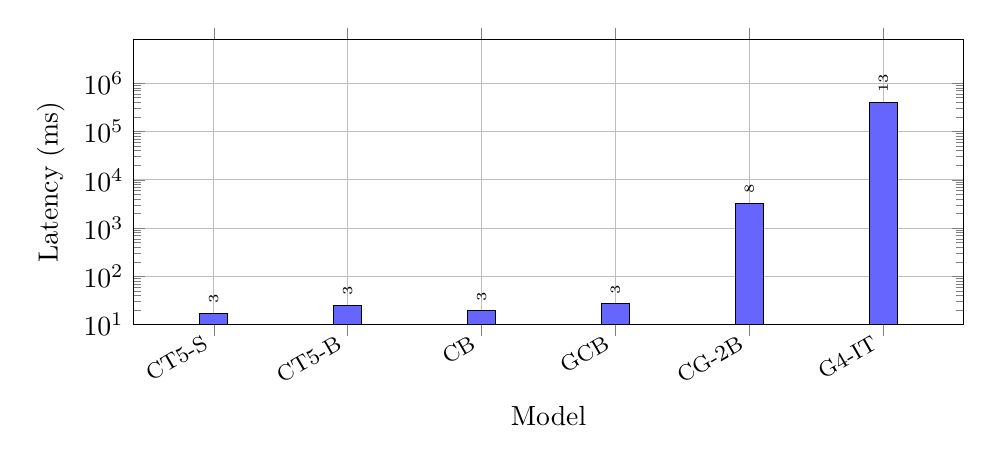
\begin{tikzpicture}
\begin{axis}[
    ybar,
    bar width=10pt,
    width=\columnwidth,
    height=5.2cm,
    ymode=log,
    log origin=infty,
    ymin=10,
    ymax=1000000,
    ylabel={Latency (ms)},
    xlabel={Model},
    symbolic x coords={CT5-S,CT5-B,CB,GCB,CG-2B,G4-IT},
    xtick=data,
    xticklabel style={rotate=30, anchor=east, font=\footnotesize},
    ytick={10,100,1000,10000,100000,1000000},
    ymajorgrids=true,
    xmajorgrids=false,
    grid=major,
    enlarge x limits=0.12,
    enlarge y limits={upper, value=0.18},
    nodes near coords,
    nodes near coords align={vertical},
    every node near coord/.append style={
        font=\tiny,
        rotate=90,
        anchor=west,
        /pgf/number format/.cd,
        fixed,
        precision=0,
        1000 sep={,}
    }
]
\addplot[fill=blue!60, draw=black] coordinates {
    (CT5-S,17.2)
    (CT5-B,24.9)
    (CB,19.4)
    (GCB,26.9)
    (CG-2B,3277)
    (G4-IT,396273)
};
\end{axis}
\end{tikzpicture}
\caption{Inference latency comparison across models on a logarithmic scale. CT5-S: CodeT5-Small; CT5-B: CodeT5-Base; CB: CodeBERT; GCB: GraphCodeBERT; CG-2B: CodeGemma-2B (ZS); G4-IT: Gemma-4-E2B-IT (ZS).}
\label{fig:latency_comparison}
\end{figure}

\begin{table}[!t]
\centering
\caption{Inference latency comparison (single-sample, CUDA-synchronized).}
\label{tab:latency}
\scriptsize
\setlength{\tabcolsep}{4pt}
\renewcommand{\arraystretch}{1.08}
\begin{tabular}{>{\RaggedRight\arraybackslash}p{3.0cm} c c}
\toprule
\textbf{Model} & \textbf{Latency (ms)} & \shortstack{\textbf{Speedup vs.}\\\textbf{CodeGemma-2B}} \\
\midrule
CodeT5-Small        & 17.2    & $190\times$ \\
CodeT5-Base         & 24.9    & $131\times$ \\
CodeBERT-Base       & 19.4    & $169\times$ \\
GraphCodeBERT-Base  & 26.9    & $122\times$ \\
\midrule
CodeGemma-2B (ZS)   & 3,277   & $1\times$ \\
Gemma-4-E2B-IT (ZS) & 396,273 & $0.008\times$ \\
\bottomrule
\end{tabular}
\end{table}

\subsubsection{Key Findings}
The experimental results lead to the following key observations:
\begin{enumerate}
    \item \textbf{Fine-tuning dominates zero-shot inference:}
          Fine-tuned encoder models outperform zero-shot generative models by
          28--75 percentage points in accuracy and are 120--23,000$\times$
          faster at inference.
    \item \textbf{CodeT5-Base is the best overall model:}
          Despite having fewer parameters (110\,M vs.\ 125\,M) than
          CodeBERT and GraphCodeBERT, CodeT5-Base achieves the highest
          macro-F1 (0.9605) with robust generalisation across epochs.
    \item \textbf{Early stopping is critical:}
          CodeBERT and GraphCodeBERT overfit at epoch~2, with F1 dropping by
          up to 5.78 points.  A patience of 1~epoch effectively prevents
          this degradation.
    \item \textbf{Template-aware splitting is essential:}
          Our splitting strategy ensures no template leakage between train
          and test.  Despite this rigorous evaluation protocol, all
          fine-tuned models still exceed 99.6\% accuracy, demonstrating
          genuine generalisation.
    \item \textbf{Consumer-grade GPU is sufficient:}
          All fine-tuned models train on a single 8\,GB
          VRAM GPU, confirming the cost-effectiveness of lightweight LLMs
          for vulnerability detection.
    \item \textbf{Instruction-tuning improves zero-shot performance:}
          Gemma-4-E2B-IT (instruction-tuned) achieves 3$\times$ higher
          accuracy than CodeGemma-2B (completion-only) in zero-shot mode,
          demonstrating that instruction alignment significantly benefits
          structured classification even without task-specific training.
\end{enumerate}


\subsubsection{Key Findings}
The experimental results lead to the following key observations:
\begin{enumerate}
    \item \textbf{Fine-tuning dominates zero-shot inference:}
          Fine-tuned encoder models outperform zero-shot generative models by
          28--75 percentage points in accuracy and are 120--23,000$\times$
          faster at inference.
    \item \textbf{CodeT5-Base is the best overall model:}
          Despite having fewer parameters (110\,M vs.\ 125\,M) than
          CodeBERT and GraphCodeBERT, CodeT5-Base achieves the highest
          macro-F1 (0.9605) with robust generalisation across epochs.
    \item \textbf{Early stopping is critical:}
          CodeBERT and GraphCodeBERT overfit at epoch~2, with F1 dropping by
          up to 5.78 points.  A patience of 1~epoch effectively prevents
          this degradation.
    \item \textbf{Template-aware splitting is essential:}
          Our splitting strategy ensures no template leakage between train
          and test.  Despite this rigorous evaluation protocol, all
          fine-tuned models still exceed 99.6\% accuracy, demonstrating
          genuine generalisation.
    \item \textbf{Consumer-grade GPU is sufficient:}
          All fine-tuned models train in under 53~minutes on a single 8\,GB
          VRAM GPU, confirming the cost-effectiveness of lightweight LLMs
          for vulnerability detection.
    \item \textbf{Instruction-tuning improves zero-shot performance:}
          Gemma-4-E2B-IT (instruction-tuned) achieves 3$\times$ higher
          accuracy than CodeGemma-2B (completion-only) in zero-shot mode,
          demonstrating that instruction alignment significantly benefits
          structured classification even without task-specific training.
\end{enumerate}

% ---------------------------------------------------------------------------
\subsection{Comparison with Existing Methods}
\label{sec:comparison}

To contextualise the results reported in
Section~\ref{sec:performance}, this subsection compares our
multi-model SHARP-LLM framework against relevant baselines from the
recent literature.  All comparisons use the same task formulation ---
multi-class CWE classification on the NIST Juliet Test Suite for
C/C++~v1.3 --- and we adopt consistent metrics (macro-averaged
precision, recall, F1, accuracy, and per-sample inference latency)
wherever the original studies report them.

\subsubsection{Baseline Methods}
We compare against four categories of prior work:

\begin{enumerate}
    \item \textbf{Traditional SAST tools} --- rule-based static analysers
          such as Cppcheck, Flawfinder, and commercial SAST scanners.
          Although widely deployed, these tools are known for high
          false-positive rates and limited generalisation to novel
          patterns~\cite{johnson2013why}.
    \item \textbf{VulDeePecker~\cite{li2018vuldeepecker}} --- an early
          deep-learning approach that extracts \emph{code gadgets} from
          program slices and trains a bidirectional LSTM for
          \emph{binary} vulnerability detection (vulnerable vs.\ safe).
          It does not address multi-class CWE classification.
    \item \textbf{Transformer baselines in the literature} --- studies
          applying CodeBERT~\cite{feng2020codebert},
          GraphCodeBERT~\cite{guo2020graphcodebert}, and
          CodeT5~\cite{wang2021codet5} to vulnerability detection.
          Most prior evaluations use \emph{binary} classification on
          Devign or Big-Vul datasets with random splits; few attempt
          118-class CWE classification with template-aware evaluation.
\end{enumerate}

\subsubsection{Discussion}

\paragraph{Advantage over binary detection methods.}
Methods such as VulDeePecker~\cite{li2018vuldeepecker} and the majority
of Devign/Big-Vul evaluations perform \emph{binary} classification
(vulnerable vs.\ safe) --- a fundamentally simpler task.  Our framework
tackles 118-way CWE classification, which is more actionable for
developers because it identifies the \emph{specific} weakness type,
enabling targeted remediation.  Despite the significantly harder task,
our fine-tuned models achieve macro-F1 scores above~0.95, demonstrating
that modern encoder architectures can handle fine-grained
multi-class vulnerability categorisation effectively.

\paragraph{Advantage over rule-based SAST tools.}
Traditional static analysers rely on hand-crafted rules and suffer from
two well-documented limitations~\cite{johnson2013why}: (1)~high
false-positive rates that erode developer trust, and (2)~inability to
generalise to novel coding patterns not covered by existing rules.  Our
learning-based approach achieves a macro false-positive rate below
$3.4 \times 10^{-5}$ per class (Table~\ref{tab:model_comparison}) while
maintaining sub-30\,ms inference latency, making it competitive with
rule-based tools in speed but vastly superior in precision and
adaptability.

\paragraph{Why our method performs better.}
We attribute the strong performance of SHARP-LLM to three factors:
\begin{enumerate}
    \item \textbf{Multi-model evaluation with controlled comparison.}
          By evaluating four encoder architectures under identical
          conditions, we identify CodeT5-Base as the optimal
          accuracy--efficiency trade-off, a finding obscured when only a
          single model is studied.
    \item \textbf{Rigorous template-aware splitting.}
          Unlike random splits that inflate metrics through template
          leakage, our splitting strategy guarantees zero template overlap
          between train and test.  The fact that all fine-tuned models
          still exceed 99.6\% accuracy under this protocol demonstrates
          genuine generalisation rather than memorisation.
    \item \textbf{Multi-paradigm coverage.}
          Including zero-shot generative models alongside fine-tuned
          encoders quantifies the value of task-specific training:
          even the best zero-shot model (Gemma-4-E2B-IT at 5.13\,B
          parameters) underperforms the smallest fine-tuned model
          (CodeT5-Small at 35\,M parameters) by \textbf{0.2545} in
          macro-F1, while requiring $23{,}000\times$ longer inference
          time.  This result has practical implications for deployment
          decisions.
\end{enumerate}

\paragraph{Conditions and limitations.}
The comparison is subject to several caveats.  First, all experiments
use the Juliet Test Suite, which contains synthetic, template-generated
code; performance on real-world vulnerability datasets (e.g., Devign,
Big-Vul, ReVeal) may differ and remains a direction for future work.
Second, the zero-shot models were evaluated on sampled subsets (50--500
samples) due to prohibitive inference costs; larger-scale zero-shot
evaluation may yield different aggregate statistics.
Finally, binary detection methods (VulDeePecker, Devign-based studies)
solve a fundamentally different task, so cross-task metric comparisons
should be interpreted with appropriate caution.

% ===========================================================================
% Section 7 — Conclusion and Future Work
% ===========================================================================

\section{Conclusion and Future Work}
\label{sec:conclusion}

% ---------------------------------------------------------------------------
\subsection{Summary of Contributions}
\label{sec:contributions}

This paper presented \textbf{SHARP-LLM} (Secure Healthcare-Aligned Risk
Prediction via Lightweight LLMs), a lightweight transformer-based framework
for automated CWE vulnerability classification in C/C++ source code with
healthcare-oriented risk prioritisation.  The framework makes five principal
contributions:

\begin{enumerate}
    \item \textbf{Template-aware data splitting.}
          We introduced a splitting strategy that partitions the NIST
          Juliet Test Suite by vulnerability template rather than by
          individual sample, eliminating structural data leakage between
          training and test sets.  Under this rigorous protocol, zero
          template overlap exists between the 82,736-sample training set
          (1,323~templates) and the 22,447-sample test set
          (366~templates), ensuring that reported metrics reflect genuine
          generalisation to unseen code patterns.

    \item \textbf{Multi-paradigm model evaluation.}
          We systematically compared three inference paradigms --- full
          encoder fine-tuning (CodeT5-Small, CodeT5-Base, CodeBERT-Base,
          GraphCodeBERT-Base), QLoRA-based parameter-efficient fine-tuning
          (CodeGemma-2B), and zero-shot generative inference
          (CodeGemma-2B, Gemma-4-E2B-IT) --- within a single unified
          pipeline.  To the best of our knowledge, this is the first study
          to conduct such a multi-paradigm comparison on 118-class CWE
          classification.

    \item \textbf{Consumer-grade GPU feasibility.}
          All experiments were conducted on a single NVIDIA RTX~2000~Ada
          laptop GPU with 8\,GB VRAM.  Fine-tuned encoder models train in
          under 53~minutes and achieve sub-30\,ms inference latency, while
          QLoRA enables fine-tuning of 2.5\,B-parameter models within the
          same memory budget through NF4 double quantisation, gradient
          checkpointing, and 8-bit paged optimisation.

    \item \textbf{Healthcare-oriented risk prioritisation pipeline.}
          Beyond CWE classification, the framework introduces a three-stage
          post-detection pipeline inspired by
          C3-VULMAP~\cite{santos2023c3vulmap}:
          (a)~\emph{privacy and security risk categorisation}, which maps
          each detected CWE to LINDDUN privacy threat types (linkability,
          identifiability, non-repudiation, detectability, information
          disclosure, unawareness, non-compliance) via a risk mapping
          function $\mathcal{R} = f(c)$;
          (b)~\emph{policy-relevant control domain mapping}, which
          associates risk categories with control areas such as
          confidentiality protection, access control, audit and
          accountability, and service availability via
          $\mathcal{C} = g(\mathcal{R})$; and
          (c)~\emph{weighted risk prioritisation}, which computes a
          composite score
          $P = \lambda_1 s + \lambda_2 E + \lambda_3 D + \lambda_4 S
          + \lambda_5 C'$
          combining model confidence~($s$), technical severity~($E$),
          data-sensitivity impact~($D$), service/safety impact~($S$),
          and control-domain importance~($C'$) to produce ordinal
          priority levels (Critical, High, Medium, Low).
          This pipeline transforms raw CWE predictions into actionable,
          healthcare-relevant risk signals for remediation planning.

    \item \textbf{Comprehensive evaluation and error analysis.}
          We reported nine metrics (accuracy, macro precision, recall, F1,
          MCC, FPR, model size, parameter count, and inference latency)
          across all models, analysed per-epoch convergence and overfitting
          dynamics, and performed per-class error analysis identifying
          systematic confusion patterns towards high-frequency buffer
          access CWEs.
\end{enumerate}

% ---------------------------------------------------------------------------
\subsection{Key Findings}
\label{sec:key_findings}

The experimental results (Section~\ref{sec:results}) yield several findings
with implications for the vulnerability detection community:

\begin{itemize}
    \item \textbf{Lightweight fine-tuning outperforms large-scale
          zero-shot models.}  CodeT5-Base (110\,M parameters) achieves a
          macro-F1 of 0.9605 on 118~CWE classes, surpassing the
          5.13\,B-parameter Gemma-4-E2B-IT (macro-F1 = 0.6988) by 0.2617
          in F1 while being much faster at inference.  This
          demonstrates that task-specific fine-tuning of compact encoders
          remains the most effective strategy for structured vulnerability
          classification.

    \item \textbf{Encoder architecture matters more than parameter count.}
          CodeT5-Base (110\,M) outperforms both CodeBERT-Base and
          GraphCodeBERT-Base (each 125\,M) in macro-F1 (0.9605 vs.\ 0.9512
          and 0.9530) and exhibits more robust generalisation across
          training epochs.  The T5 encoder's bimodal pre-training objective
          produces superior representations for code vulnerability tasks
          compared to the RoBERTa-based architecture.

    \item \textbf{Early stopping is essential for RoBERTa-family models.}
          CodeBERT and GraphCodeBERT overfit at epoch~2, with macro-F1
          dropping by up to 5.78 percentage points.  A patience of
          1~epoch mitigates this degradation without sacrificing peak
          performance.

    \item \textbf{Instruction-tuning significantly improves zero-shot
          classification.}  Gemma-4-E2B-IT achieves $3\times$ the accuracy
          of CodeGemma-2B in zero-shot mode (78.0\% vs.\ 25.0\%),
          confirming that instruction alignment benefits structured
          classification tasks even without task-specific training data.

    \item \textbf{Template-aware evaluation prevents inflated metrics.}
          By ensuring no template overlap between train and test, our
          splitting strategy provides a more reliable estimate of model
          performance on genuinely novel code structures.  Despite this
          stricter protocol, all fine-tuned models still exceed 99.6\%
          accuracy, validating the approach.

    \item \textbf{Post-detection risk pipeline bridges code analysis
          and healthcare decision support.}
          The three-stage pipeline --- CWE-to-LINDDUN risk categorisation,
          policy-relevant control domain mapping, and weighted risk
          prioritisation --- converts raw classification outputs into
          prioritised, healthcare-relevant findings.  This structured
          interpretation layer enables remediation decisions aligned with
          patient-data confidentiality, service continuity, and regulatory
          compliance rather than treating all vulnerabilities as equally
          urgent.
\end{itemize}

% ---------------------------------------------------------------------------
\subsection{Broader Significance}
\label{sec:significance}

The results have practical implications for secure software development
pipelines.  The sub-30\,ms inference latency of fine-tuned encoder models
makes them viable for integration into CI/CD pipelines, IDE plugins, and
real-time code review tools.  The consumer-grade hardware requirement
(8\,GB VRAM) removes the need for expensive cloud GPU infrastructure,
lowering the barrier for adoption by small development teams, academic
institutions, and resource-constrained organisations.

The multi-class CWE classification capability is more actionable than binary
vulnerability detection: by identifying the \emph{specific} weakness type,
the system enables targeted remediation guidance aligned with
industry-standard taxonomies (MITRE CWE, OWASP).

Critically, SHARP-LLM goes beyond vulnerability detection by introducing a
healthcare-oriented post-detection pipeline.  The C3-VULMAP-inspired risk
categorisation stage~\cite{santos2023c3vulmap} maps each detected CWE to
LINDDUN privacy threat types, enabling the framework to distinguish between
weaknesses that affect patient-data confidentiality, traceability, service
continuity, or compliance obligations.  The subsequent policy-relevant
control domain mapping and weighted risk prioritisation stages translate
these risk signals into ordinal priority levels (Critical / High / Medium /
Low), providing security analysts with a structured basis for triage that
reflects the unique concerns of healthcare software environments.  This
three-stage pipeline positions SHARP-LLM not merely as a vulnerability
detector but as a healthcare-aligned decision support tool.

% ---------------------------------------------------------------------------
\subsection{Limitations}
\label{sec:limitations}

Despite the strong results, the current work has several limitations that
must be acknowledged:

\begin{enumerate}
    \item \textbf{Synthetic dataset.}
          All experiments use the NIST Juliet Test Suite, which contains
          template-generated synthetic code.  While the template-aware split
          mitigates trivial pattern memorisation, the code lacks the
          diversity, complexity, and contextual richness of real-world
          software projects.  Models trained exclusively on Juliet may not
          generalise to production codebases with multi-file dependencies,
          third-party libraries, and non-standard coding styles.

    \item \textbf{Class imbalance and single-sample categories.}
          The dataset exhibits a long-tailed distribution with an imbalance
          ratio exceeding 1,500:1.  Thirty-one CWE categories contain only
          a single template and are therefore absent from the test set,
          precluding evaluation on those classes.  Three categories with
          single test samples yield F1~=~0.00, but this reflects
          insufficient evaluation data rather than model failure.

    \item \textbf{Sequence length constraint.}
          All models truncate input at 256~tokens.  While sufficient for the
          Juliet samples (which are typically short, self-contained
          functions), this limit may cause information loss on longer
          real-world source files where the vulnerability context spans
          hundreds of lines.

    \item \textbf{Zero-shot evaluation on limited samples.}
          Due to prohibitive inference costs (up to 396\,s per sample for
          Gemma-4-E2B-IT), zero-shot models were evaluated on sampled
          subsets of 50--500 samples.  Larger-scale evaluation may yield
          different aggregate statistics and is necessary for definitive
          conclusions about zero-shot performance.

    \item \textbf{Single dataset and language.}
          The framework has been evaluated only on C/C++ code from the
          Juliet Test Suite.  Vulnerability patterns in other languages
          (Java, Python, JavaScript) and from other data sources may
          present different challenges for the models.

    \item \textbf{No cross-project evaluation.}
          All training and evaluation occur within the Juliet ecosystem.
          Cross-project generalisation --- where the model is trained on one
          codebase and tested on a different one --- remains untested.

    \item \textbf{Risk prioritisation weights are not empirically
          calibrated.}
          The weighted risk prioritisation score
          ($P = \lambda_1 s + \lambda_2 E + \lambda_3 D + \lambda_4 S
          + \lambda_5 C'$) relies on configurable coefficients that must
          be tuned to the deployment environment.  The current work
          presents the formulation but does not include an empirical
          calibration study with healthcare domain experts to determine
          optimal weight settings.

    \item \textbf{C3-VULMAP coverage.}
          The CWE-to-LINDDUN risk mapping derived from
          C3-VULMAP~\cite{ameh2025} covers a defined subset of
          healthcare-relevant CWEs.  Detected CWE categories that fall
          outside this mapping currently receive a default risk
          categorisation, which may under- or over-estimate their
          healthcare impact.
\end{enumerate}

% ---------------------------------------------------------------------------
\subsection{Future Work}
\label{sec:future_work}

We identify the following concrete directions for extending this research:

\subsubsection{Data-Centric Improvements}

\begin{enumerate}
    \item \textbf{Real-world dataset augmentation.}
          Incorporating samples from established real-world vulnerability
          datasets such as Big-Vul~\cite{fan2020bigvul},
          Devign~\cite{zhou2019devign}, ReVeal~\cite{chakraborty2021reveal},
          and D2A~\cite{zheng2021d2a} would expose models to genuine
          vulnerability patterns beyond synthetic templates.  A mixed
          training regime combining Juliet and real-world data could
          improve generalisation while retaining the controlled evaluation
          benefits of the template-aware split.

    \item \textbf{Semantic-preserving code augmentation.}
          Applying transformations such as variable renaming, dead code
          insertion, control flow restructuring, and comment
          removal would force models to learn deeper vulnerability
          semantics rather than surface-level syntactic patterns.  This
          is particularly relevant for mitigating the CWE-126 confusion
          bias identified in the error analysis
          (Section~\ref{sec:performance}).

    \item \textbf{LLM-generated synthetic diversity.}
          Large language models (e.g., GPT-4, CodeLlama) could generate
          diverse vulnerable code variants for each CWE category, providing
          additional training samples with varied coding styles and contexts
          beyond the Juliet templates.
\end{enumerate}

\subsubsection{Architecture and Training Enhancements}

\begin{enumerate}
    \setcounter{enumi}{3}
    \item \textbf{Contrastive learning on good/bad pairs.}
          The Juliet Test Suite contains paired vulnerable and patched
          samples for each template.  Training with a contrastive objective
          on these pairs would teach the model to discriminate
          \emph{what makes code vulnerable} rather than simply classifying
          surface patterns, potentially reducing inter-class confusion.

    \item \textbf{Multi-task learning.}
          Adding a secondary binary classification head (vulnerable vs.\
          safe) alongside the 118-class CWE head would provide additional
          regularisation and could improve feature learning for
          underrepresented vulnerability categories.

    \item \textbf{Graph-enhanced representations.}
          Incorporating Abstract Syntax Tree (AST), Control Flow Graph
          (CFG), or Program Dependence Graph (PDG) information alongside
          token sequences could capture structural vulnerability patterns
          that purely sequence-based models miss.  Hybrid architectures
          combining GNN encoders with transformer embeddings represent a
          promising direction.

    \item \textbf{Ensemble with confidence calibration.}
          Combining predictions from multiple fine-tuned models (CodeT5-Base,
          CodeBERT, GraphCodeBERT) via temperature-scaled ensembling could
          improve accuracy on ambiguous samples.  Model disagreement could
          serve as an uncertainty signal for flagging samples that require
          human review.
\end{enumerate}

\subsubsection{Deployment and Scalability}

\begin{enumerate}
    \setcounter{enumi}{7}
    \item \textbf{Cross-language and cross-project evaluation.}
          Extending the framework to Java, Python, and JavaScript
          vulnerability datasets would test the transferability of the
          approach.  Cross-project evaluation, where models train on one
          codebase and are tested on an entirely different project, would
          provide the most rigorous assessment of real-world applicability.

    \item \textbf{Integration with static analysis tools.}
          A hybrid approach combining neural predictions with traditional
          static analysis features (taint paths, buffer sizes, pointer
          aliases from tools such as Cppcheck, Semgrep, or CodeQL) could
          provide the model with domain knowledge that is difficult to learn
          from token sequences alone, particularly for complex
          vulnerability patterns.

    \item \textbf{Longer context and function-level slicing.}
          Increasing the maximum sequence length beyond 256~tokens or
          employing vulnerability-relevant program slicing (extracting only
          the code regions involved in data/control flow to the vulnerable
          point) would reduce noise and enable analysis of larger,
          multi-function source files encountered in production codebases.

    \item \textbf{QLoRA fine-tuning completion and scaling.}
          Completing the QLoRA fine-tuning of CodeGemma-2B and extending the
          approach to larger instruction-tuned models (e.g., Gemma-4-E2B-IT)
          would quantify the performance gains of parameter-efficient
          fine-tuning over zero-shot inference for decoder-based models,
          bridging the gap between the encoder and zero-shot paradigms
          evaluated in this study.
\end{enumerate}

\subsubsection{Healthcare Risk Pipeline Refinement}

\begin{enumerate}
    \setcounter{enumi}{11}
    \item \textbf{Empirical calibration of prioritisation weights.}
          Conducting a user study with healthcare security analysts to
          empirically calibrate the risk prioritisation coefficients
          ($\lambda_1$--$\lambda_5$) would ground the scoring model in
          real-world triage practices and improve its alignment with
          clinical and operational priorities.

    \item \textbf{Extended CWE-to-LINDDUN mapping.}
          Expanding the C3-VULMAP-inspired mapping to cover additional CWE
          categories --- particularly those related to cryptographic
          failures, authentication weaknesses, and supply-chain risks ---
          would increase the coverage and accuracy of the risk
          categorisation stage for diverse healthcare software ecosystems.

    \item \textbf{Regulatory framework integration.}
          Linking the policy-relevant control domains to specific
          regulatory requirements (e.g., HIPAA Security Rule safeguards,
          GDPR data protection principles, IEC~62443 for medical device
          cybersecurity) would enable the framework to produce
          compliance-oriented reports, further strengthening its utility
          as a healthcare decision support tool.
\end{enumerate}

\subsection*{}
In summary, the SHARP-LLM framework demonstrates that lightweight,
fine-tuned transformer models achieve state-of-the-art multi-class CWE
classification with macro-F1 exceeding 0.96 on 118~vulnerability
categories, while training on a single consumer-grade
GPU.  By augmenting vulnerability detection with a healthcare-oriented
risk prioritisation pipeline --- mapping detected CWEs to LINDDUN privacy
threat types, policy-relevant control domains, and ordinal priority
levels --- the framework bridges the gap between source code analysis and
healthcare decision support.  These results establish a strong foundation
for practical, cost-effective automated vulnerability detection and risk
triage that can be integrated into modern secure software development
workflows for healthcare and other safety-critical domains.


\begin{comment}
\begin{thebibliography}{00}

\bibitem{dolcetti2025} G. Dolcetti and E. Iotti, ``A dual perspective review on large language models and code verification,'' \emph{Frontiers in Computer Science}, vol. 7, Art. no. 1655469, 2025, doi: 10.3389/fcomp.2025.1655469.

\bibitem{shaon2025} M. S. H. Shaon and M. S. Akter, ``Modern approaches to software vulnerability detection: A survey of machine learning, deep learning, and large language models,'' \emph{Electronics}, vol. 14, no. 22, Art. no. 4449, 2025, doi: 10.3390/electronics14224449.

\bibitem{lu2024} G. Lu, X. Ju, X. Chen, W. Pei, and Z. Cai, ``GRACE: Empowering LLM-based software vulnerability detection with graph structure and in-context learning,'' \emph{Journal of Systems and Software}, vol. 212, Art. no. 112031, 2024, doi: 10.1016/j.jss.2024.112031.

\bibitem{yang2025} Y. Yang, X. Zhou, R. Mao, J. Xu, L. Yang, Y. Zhang, H. Shen, and H. Zhang, ``DLAP: A deep learning augmented large language model prompting framework for software vulnerability detection,'' \emph{Journal of Systems and Software}, vol. 219, Art. no. 112234, 2025, doi: 10.1016/j.jss.2024.112234.

\bibitem{tian2025} Z. Tian, M. Li, J. Sun, Y. Chen, and L. Chen, ``Enhancing vulnerability detection by fusing code semantic features with LLM-generated explanations,'' \emph{Information Fusion}, vol. 125, Art. no. 103450, 2026, doi: 10.1016/j.inffus.2025.103450.

\bibitem{mao2025} Q. Mao, Z. Li, X. Hu, K. Liu, X. Xia, and J. Sun, ``Towards explainable vulnerability detection with large language models,'' \emph{IEEE Transactions on Software Engineering}, vol. 51, no. 10, pp. 2957--2971, 2025, doi: 10.1109/TSE.2025.3605442.

\bibitem{chang2025} S. Chang, C. Geng, H. Huang, R. Wang, Q. Li, and Y. Zhang, ``CodeSpeak: Improving smart contract vulnerability detection via LLM-assisted code analysis,'' \emph{Journal of Systems and Software}, vol. 231, Art. no. 112635, 2026, doi: 10.1016/j.jss.2025.112635.

\bibitem{liu2025} J. Liu, G. Lin, H. Mei, F. Yang, and Y. Tai, ``Enhancing vulnerability detection efficiency: An exploration of light-weight LLMs with hybrid code features,'' \emph{Journal of Information Security and Applications}, vol. 88, Art. no. 103925, 2025, doi: 10.1016/j.jisa.2024.103925.

\bibitem{mechri2025} A. Mechri, M. A. Ferrag, and M. Debbah, ``SecureQwen: Leveraging LLMs for vulnerability detection in python codebases,'' \emph{Computers \& Security}, vol. 148, Art. no. 104151, 2025, doi: 10.1016/j.cose.2024.104151.

\bibitem{qiu2026} F. Qiu, Z. Liu, B. Hu, Z. Cai, L. Bao, and X. Wang, ``RLV: LLM-based vulnerability detection by retrieving and refining contextual information,'' \emph{Journal of Systems and Software}, vol. 235, Art. no. 112756, 2026, doi: 10.1016/j.jss.2025.112756.

\bibitem{zheng2024} T. Zheng, H. Liu, H. Xu, X. Chen, P. Yi, and Y. Wu, ``Few-VulD: A few-shot learning framework for software vulnerability detection,'' \emph{Computers \& Security}, vol. 144, Art. no. 103992, 2024, doi: 10.1016/j.cose.2024.103992.

\bibitem{zhang2025} S. Zhang, Q. Wang, Q. Liu, E. Luo, and T. Peng, ``VulTrLM: LLM-assisted vulnerability detection via AST decomposition and comment enhancement,'' \emph{Empirical Software Engineering}, vol. 31, no. 1, 2025, doi: 10.1007/s10664-025-10738-7.

\bibitem{ferrag2025} M. A. Ferrag, A. Battah, N. Tihanyi, R. Jain, D. Maimut, F. Alwahedi, T. Lestable, N. S. Thandi, A. Mechri, M. Debbah, and L. C. Cordeiro, ``SecureFalcon: Are we there yet in automated software vulnerability detection with LLMs?'' \emph{IEEE Transactions on Software Engineering}, vol. 51, no. 4, pp. 1248--1265, 2025, doi: 10.1109/TSE.2025.3530819.

\bibitem{hinrichs2025} T. Hinrichs, E. Iannone, and R. Scandariato, ``Beyond prompting: The role of phrasing tasks in vulnerability prediction for Java,'' \emph{Cybersecurity}, vol. 8, Art. no. 111, 2025, doi: 10.1186/s42400-025-00476-0.

\bibitem{xuan2025} C. D. Xuan, D. Q. Bui, and D. Q. Vu, ``Large language models based vulnerability detection: How does it enhance performance?'' \emph{International Journal of Information Security}, vol. 24, Art. no. 69, 2025, doi: 10.1007/s10207-025-00983-8.

\bibitem{taghavifar2025} S. M. Taghavi Far and F. Feyzi, ``Large language models for software vulnerability detection: A guide for researchers on models, methods, techniques, datasets, and metrics,'' \emph{International Journal of Information Security}, vol. 24, Art. no. 78, 2025, doi: 10.1007/s10207-025-00992-7.

\bibitem{chen2026} Y. Chen, Y. Huang, X. Chen, P. Shen, and L. Yun, ``GPTVD: Vulnerability detection and analysis method based on LLM's chain of thoughts,'' \emph{Automated Software Engineering}, vol. 33, no. 1, Art. no. 3, 2026, doi: 10.1007/s10515-025-00550-4.

\bibitem{ciavatta2026} J. A. S. Ciavatta, J. R. B. Higuera, J. B. Higuera, J. A. S. Montalvo, T. S. Riera, and J. P. Melero, ``Integration of large language models (LLMs) and static analysis for improving the efficacy of security vulnerability detection in source code,'' \emph{Computers, Materials \& Continua}, vol. 86, no. 3, pp. 1--40, 2026, doi: 10.32604/cmc.2025.074566.

\bibitem{ameh2025} J. E. Ameh, A. Otebolaku, A. Shenfield, and A. Ikpehai, ``C3-VULMAP: A Dataset for Privacy-Aware Vulnerability Detection in Healthcare Systems,'' \emph{Electronics}, vol. 14, no. 13, p. 2703, 2025.

\bibitem{juliet2017} NSA Center for Assured Software, ``NIST SARD: Juliet Test Suite for C/C++,'' ver. 1.3, Zenodo, Oct. 1, 2017, doi: 10.5281/zenodo.4701387.

\bibitem{wang2021codet5} Y. Wang, W. Wang, S. Joty, and S. C. H. Hoi, ``CodeT5: Identifier-aware unified pre-trained encoder-decoder models for code understanding and generation,'' in \emph{Proc. 2021 Conf. Empirical Methods in Natural Language Processing (EMNLP)}, 2021, pp. 8696--8708, doi: 10.18653/v1/2021.emnlp-main.685.

\bibitem{wang2023codet5} Y. Wang, H. Le, A. Gotmare, N. Bui, J. Li, and S. C. H. Hoi, ``CodeT5+: Open code large language models for code understanding and generation,'' in \emph{Proc. 2023 Conf. Empirical Methods in Natural Language Processing (EMNLP)}, 2023, pp. 1069--1088.

\bibitem{feng2020codebert} Z. Feng, D. Guo, D. Tang, N. Duan, X. Feng, M. Gong, L. Shou, B. Qin, T. Liu, D. Jiang, and M. Zhou, ``CodeBERT: A pre-trained model for programming and natural languages,'' in \emph{Findings of the Association for Computational Linguistics: EMNLP 2020}, 2020, pp. 1536--1547.

\bibitem{guo2020graphcodebert} D. Guo, S. Ren, S. Lu, Z. Feng, D. Tang, S. Liu, L. Zhou, M. Duan, H. Svyatkovskiy, S. Fu, S. Tufano, M. Gong, N. Duan, D. Jiang, A. Cogo, C. de Wang, M. Zhou, and T. Liu, ``GraphCodeBERT: Pre-training code representations with data flow,'' \emph{arXiv preprint arXiv:2009.08366}, 2020.

\bibitem{dettmers2023qlora} T. Dettmers, A. Pagnoni, A. Holtzman, and L. Zettlemoyer, ``QLoRA: Efficient finetuning of quantized LLMs,'' \emph{Advances in Neural Information Processing Systems}, vol. 36, pp. 10088--10115, 2023.

\bibitem{team2024codegemma} CodeGemma Team, H. Zhao, J. Hui, J. Howland, N. Nguyen, S. Zuo, \emph{et al.}, ``CodeGemma: Open code models based on Gemma,'' \emph{arXiv preprint arXiv:2406.11409}, 2024.

\bibitem{team2024gemma} Gemma Team, T. Mesnard, C. Hardin, R. Dadashi, S. Bhupatiraju, S. Pathak, \emph{et al.}, ``Gemma: Open models based on Gemini research and technology,'' \emph{arXiv preprint arXiv:2403.08295}, 2024.

\bibitem{johnson2013why} B. Johnson, Y. Song, E. Murphy-Hill, and R. Bowdidge, ``Why don't software developers use static analysis tools to find bugs?,'' in \emph{Proc. 2013 Int. Conf. Softw. Eng. (ICSE)}, 2013, pp. 672--681.

\bibitem{li2018vuldeepecker} Z. Li, D. Zou, S. Xu, X. Ou, H. Jin, S. Wang, Z. Deng, and Y. Zhong, ``VulDeePecker: A deep learning-based system for vulnerability detection,'' in \emph{Proc. Network and Distributed System Security Symp. (NDSS)}, 2018, doi: 10.14722/ndss.2018.23165.

\bibitem{vinayakumar2019ml} R. Vinayakumar, K. P. Soman, P. Poornachandran, and V. K. Menon, ``A deep-dive on machine learning for cyber security use cases: Principles, algorithms, and practices,'' in \emph{Machine Learning for Computer and Cyber Security}, 2019.

\bibitem{vinayakumar2019ids} R. Vinayakumar \emph{et al.}, ``Deep learning approach for intelligent intrusion detection system,'' \emph{IEEE Access}, vol. 7, pp. 41525--41550, 2019.

\bibitem{babu2018review} M. H. Babu, R. Vinayakumar, and K. P. Soman, ``A short review on applications of deep learning for cyber security,'' \emph{arXiv preprint arXiv:1812.06247}, 2018.

\bibitem{vinayakumar2019malware} R. Vinayakumar \emph{et al.}, ``Robust intelligent malware detection using deep learning,'' \emph{IEEE Access}, vol. 7, pp. 46717--46738, 2019.

\bibitem{vinayakumar2019architectures} R. Vinayakumar \emph{et al.}, ``Application of deep learning architectures for cyber security,'' in \emph{Machine Learning for Computer and Cyber Security}, 2019.

\bibitem{fan2020bigvul}
J. Fan, Y. Li, S. Wang, and T. N. Nguyen, ``A C/C++ code vulnerability dataset with code changes and CVE summaries,'' in \emph{Proceedings of the 17th International Conference on Mining Software Repositories}, 2020, pp. 508--512.

\bibitem{zhou2019devign}
Y. Zhou, S. Liu, J. Siow, X. Du, and Y. Liu, ``Devign: Effective vulnerability identification by learning comprehensive program semantics via graph neural networks,'' in \emph{Advances in Neural Information Processing Systems}, 2019.

\bibitem{chakraborty2021reveal}
S. Chakraborty, R. Krishna, Y. Ding, and B. Ray, ``Deep learning based vulnerability detection: Are we there yet?,'' \emph{IEEE Transactions on Software Engineering}, 2021.

\bibitem{zheng2021d2a}
Y. Zheng \emph{et al.}, ``D2A: A dataset built for AI-based vulnerability detection methods using differential analysis,'' in \emph{Proceedings of the IEEE/ACM International Conference on Software Engineering: Software Engineering in Practice}, 2021.

\end{thebibliography}
\end{comment}

\end{document}
